\documentclass[12pt, spanish]{article}
\usepackage[spanish]{babel}
\selectlanguage{spanish}
%\usepackage{natbib}
\usepackage{url}
\usepackage[utf8x]{inputenc}
\usepackage{graphicx}
\graphicspath{{images/}}
\usepackage{parskip}
\usepackage{fancyhdr}
\usepackage{vmargin}
\usepackage{multirow}
\usepackage{float}
\usepackage{chngpage}

%Para poder hacer diagramas BNF en LaTeX
\usepackage{backnaur}
\usepackage{syntax}

\usepackage{amsfonts}

\usepackage{subcaption}

\usepackage{hyperref}
\usepackage[
    type={CC},
    modifier={by-nc-sa},
    version={4.0},
]{doclicense}

\hypersetup{
    colorlinks=true,
    linkcolor=blue,
    filecolor=magenta,
    urlcolor=cyan,
}

% para codigo
\usepackage{listings}
\usepackage[dvipsnames]{xcolor}


\lstdefinelanguage{Kotlin}{
  comment=[l]{//},
  commentstyle={\color{gray}\ttfamily},
  emph={delegate, filter, first, firstOrNull, forEach, lazy, map, mapNotNull, println, return@},
  emphstyle={\color{OrangeRed}},
  identifierstyle=\color{black},
  keywords={abstract, actual, as, as?, break, by, class, companion, continue, data, do, dynamic, else, enum, expect, false, final, for, fun, get, if, import, in, interface, internal, is, null, object, override, package, private, public, return, set, super, suspend, this, throw, true, try, typealias, val, var, vararg, when, where, while},
  keywordstyle={\color{NavyBlue}\bfseries},
  morecomment=[s]{/*}{*/},
  morestring=[b]",
  morestring=[s]{"""*}{*"""},
  ndkeywords={@Deprecated, @JvmField, @JvmName, @JvmOverloads, @JvmStatic, @JvmSynthetic, Array, Byte, Double, Float, Int, Integer, Iterable, Long, Runnable, Short, String},
  ndkeywordstyle={\color{BurntOrange}\bfseries},
  sensitive=true,
  stringstyle={\color{ForestGreen}\ttfamily},
}


%% configuración de listings

\definecolor{listing-background}{HTML}{F7F7F7}
\definecolor{listing-rule}{HTML}{B3B2B3}
\definecolor{listing-numbers}{HTML}{B3B2B3}
\definecolor{listing-text-color}{HTML}{000000}
\definecolor{listing-keyword}{HTML}{435489}
\definecolor{listing-identifier}{HTML}{435489}
\definecolor{listing-string}{HTML}{00999A}
\definecolor{listing-comment}{HTML}{8E8E8E}
\definecolor{listing-javadoc-comment}{HTML}{006CA9}

\lstdefinestyle{eisvogel_listing_style}{
  language         = python,
%$if(listings-disable-line-numbers)$
%  xleftmargin      = 0.6em,
%  framexleftmargin = 0.4em,
%$else$
  numbers          = left,
  xleftmargin      = 0em,
 framexleftmargin = 0em,
%$endif$
  backgroundcolor  = \color{listing-background},
  basicstyle       = \color{listing-text-color}\small\ttfamily{}\linespread{1.15}, % print whole listing small
  breaklines       = true,
  frame            = single,
  framesep         = 0.19em,
  rulecolor        = \color{listing-rule},
  frameround       = ffff,
  tabsize          = 4,
  numberstyle      = \color{listing-numbers},
  aboveskip        = 1.0em,
  belowskip        = 0.1em,
  abovecaptionskip = 0em,
  belowcaptionskip = 1.0em,
  keywordstyle     = \color{listing-keyword}\bfseries,
  classoffset      = 0,
  sensitive        = true,
  identifierstyle  = \color{listing-identifier},
  commentstyle     = \color{listing-comment},
  morecomment      = [s][\color{listing-javadoc-comment}]{/**}{*/},
  stringstyle      = \color{listing-string},
  showstringspaces = false,
  escapeinside     = {/*@}{@*/}, % Allow LaTeX inside these special comments
  literate         =
  {á}{{\'a}}1 {é}{{\'e}}1 {í}{{\'i}}1 {ó}{{\'o}}1 {ú}{{\'u}}1
  {Á}{{\'A}}1 {É}{{\'E}}1 {Í}{{\'I}}1 {Ó}{{\'O}}1 {Ú}{{\'U}}1
  {à}{{\`a}}1 {è}{{\'e}}1 {ì}{{\`i}}1 {ò}{{\`o}}1 {ù}{{\`u}}1
  {À}{{\`A}}1 {È}{{\'E}}1 {Ì}{{\`I}}1 {Ò}{{\`O}}1 {Ù}{{\`U}}1
  {ä}{{\"a}}1 {ë}{{\"e}}1 {ï}{{\"i}}1 {ö}{{\"o}}1 {ü}{{\"u}}1
  {Ä}{{\"A}}1 {Ë}{{\"E}}1 {Ï}{{\"I}}1 {Ö}{{\"O}}1 {Ü}{{\"U}}1
  {â}{{\^a}}1 {ê}{{\^e}}1 {î}{{\^i}}1 {ô}{{\^o}}1 {û}{{\^u}}1
  {Â}{{\^A}}1 {Ê}{{\^E}}1 {Î}{{\^I}}1 {Ô}{{\^O}}1 {Û}{{\^U}}1
  {œ}{{\oe}}1 {Œ}{{\OE}}1 {æ}{{\ae}}1 {Æ}{{\AE}}1 {ß}{{\ss}}1
  {ç}{{\c c}}1 {Ç}{{\c C}}1 {ø}{{\o}}1 {å}{{\r a}}1 {Å}{{\r A}}1
  {€}{{\EUR}}1 {£}{{\pounds}}1 {«}{{\guillemotleft}}1
  {»}{{\guillemotright}}1 {ñ}{{\~n}}1 {Ñ}{{\~N}}1 {¿}{{?`}}1
  {…}{{\ldots}}1 {≥}{{>=}}1 {≤}{{<=}}1 {„}{{\glqq}}1 {“}{{\grqq}}1
  {”}{{''}}1
}
\lstset{style=eisvogel_listing_style}


\usepackage[default]{sourcesanspro}

\setmarginsrb{2 cm}{1 cm}{2 cm}{2 cm}{1 cm}{1.5 cm}{1 cm}{1.5 cm}

\title{Guía Universitaria. Memoria Técnica\\
  \hspace{0.05cm} }
\author{Antonio David Villegas Yeguas\\
		Juan Emilio Martinez Manjon\\
		Alejandro Manzanares Lemus\\
		Juan Mota Martínez}
\date{\today}

\renewcommand*\contentsname{hola}

\makeatletter
\let\thetitle\@title
\let\theauthor\@author
\let\thedate\@date
\makeatother

\pagestyle{fancy}
\fancyhf{}
\rhead{\theauthor}
\lhead{\thetitle}
\cfoot{\thepage}

\begin{document}

%%%%%%%%%%%%%%%%%%%%%%%%%%%%%%%%%%%%%%%%%%%%%%%%%%%%%%%%%%%%%%%%%%%%%%%%%%%%%%%%%%%%%%%%%

\begin{titlepage}
    \centering
    \vspace*{0.3 cm}
    
\includegraphics[scale = 0.50]{ugr.png}\\[0.7 cm]
    %\textsc{\LARGE Universidad de Granada}\\[2.0 cm]
    \textsc{\large 4º CSI 2020/21 - Grupo 4}\\[0.5 cm]
    \textsc{\large Grado en Ingeniería Informática}\\[0.5 cm]
    \rule{\linewidth}{0.2 mm} \\[0.2 cm]
    { \huge \bfseries \thetitle}\\
    \rule{\linewidth}{0.2 mm} \\[1 cm]

    \begin{minipage}{0.4\textwidth}
        \begin{flushleft} \large
            \emph{Autores:}\\
            \theauthor\\
            \end{flushleft}
            \end{minipage}~
            \begin{minipage}{0.4\textwidth}
            \begin{flushright} \large
            \emph{Asignatura: \\
            Nuevos Paradigmas de Interacción}   \\

        \end{flushright}
    \end{minipage}\\[0.5cm]

    {\large \thedate}\\[0.5cm]
    %{\url{https://github.com/advy99/NPI/}}
    {\doclicenseThis}

    \vfill

\end{titlepage}

%%%%%%%%%%%%%%%%%%%%%%%%%%%%%%%%%%%%%%%%%%%%%%%%%%%%%%%%%%%%%%%%%%%%%%%%%%%%%%%%%%%%%%%%%

\tableofcontents
\pagebreak

\section{Diagrama de clases}

\begin{figure}[H]
	\centering
	%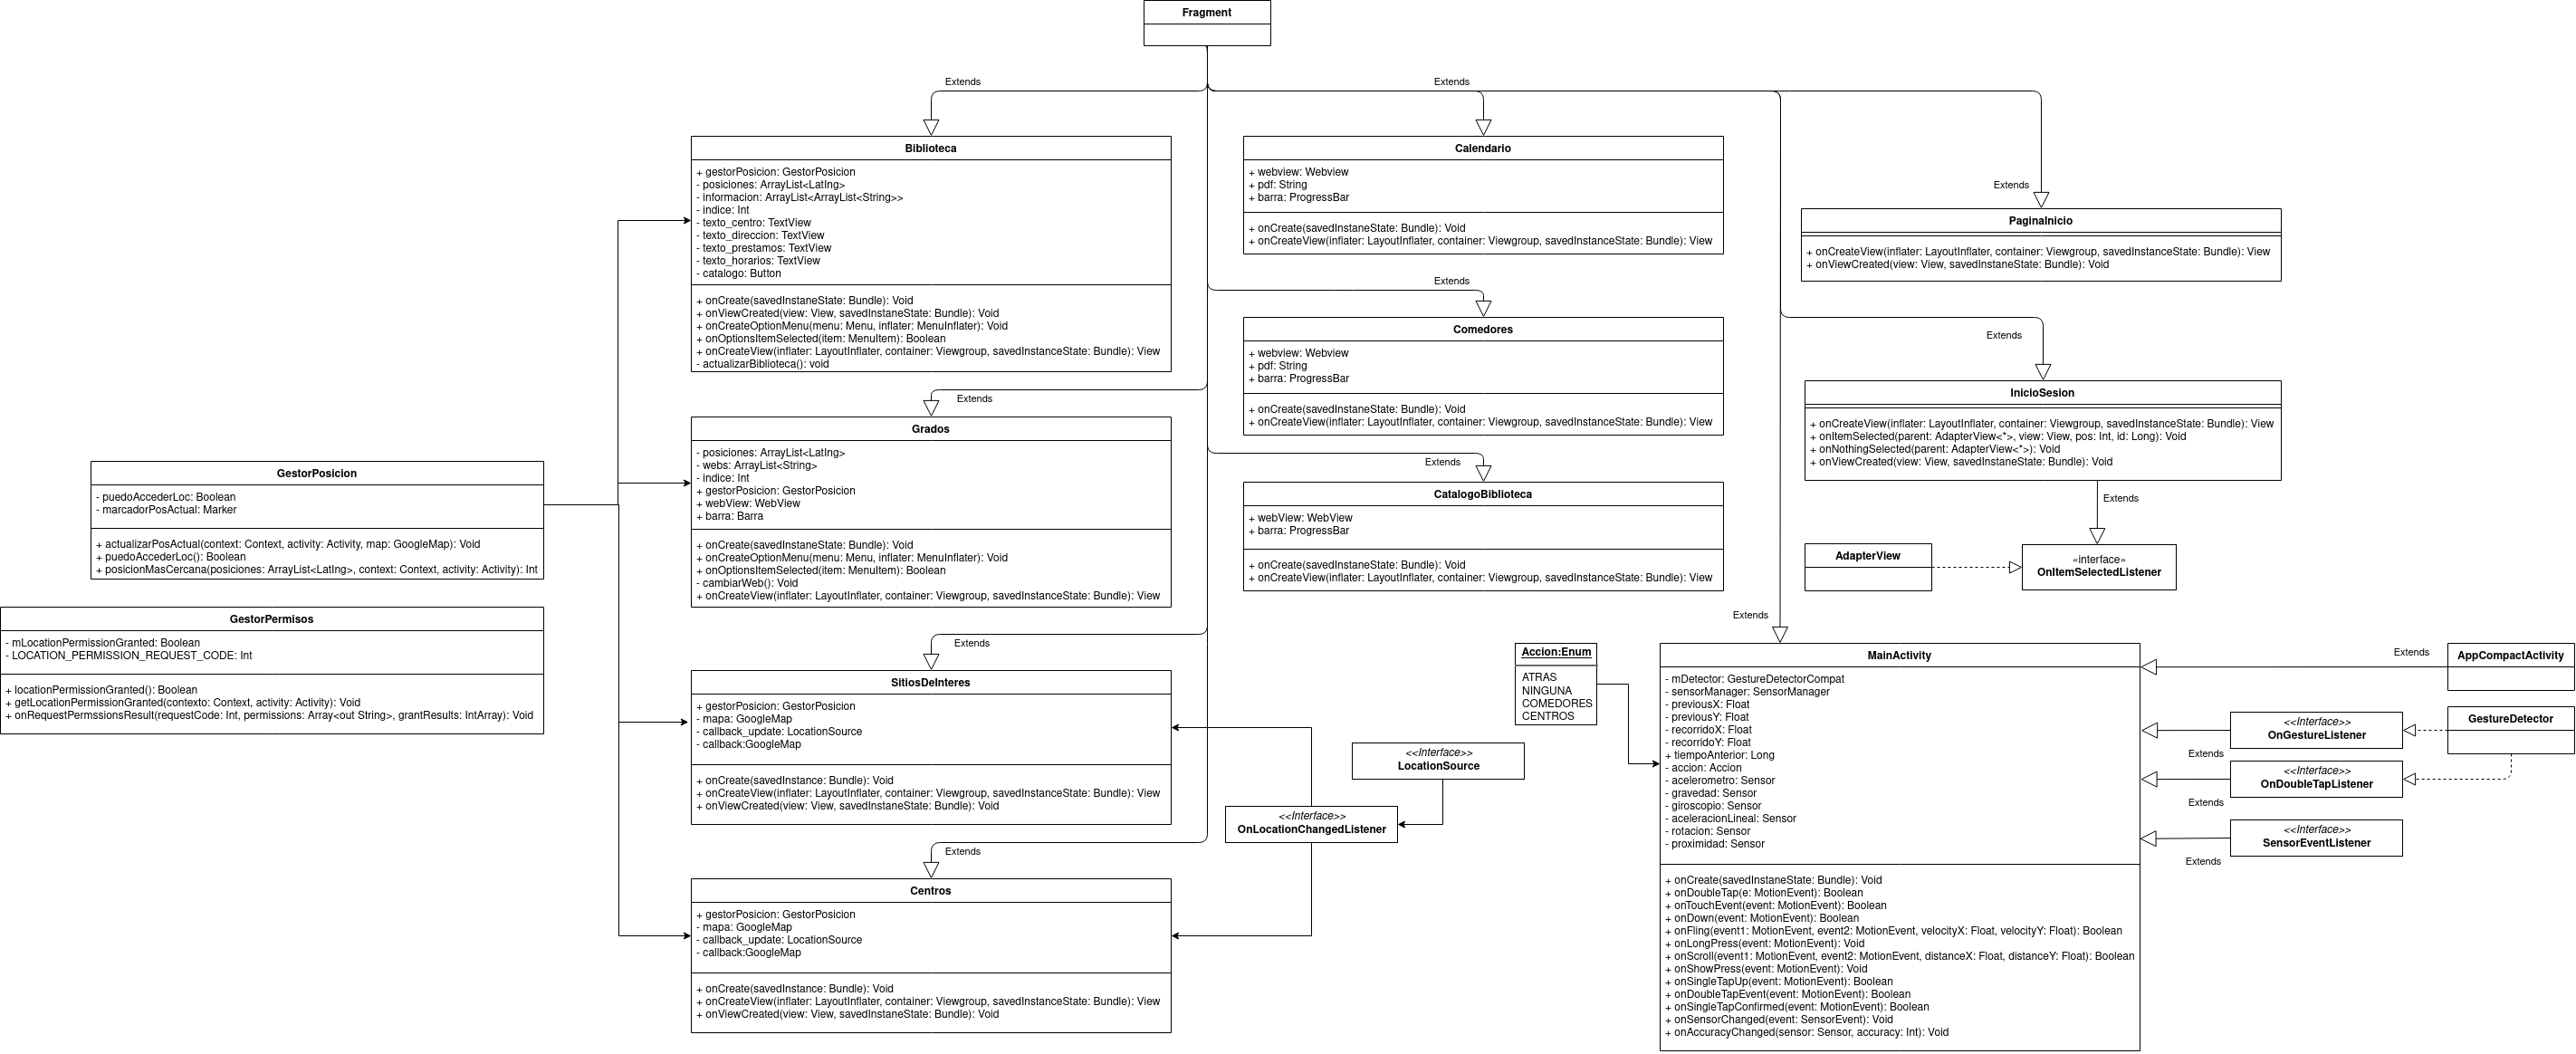
\includegraphics[width=\textheight, angle=90]{GuiaEstudiantes.png}
	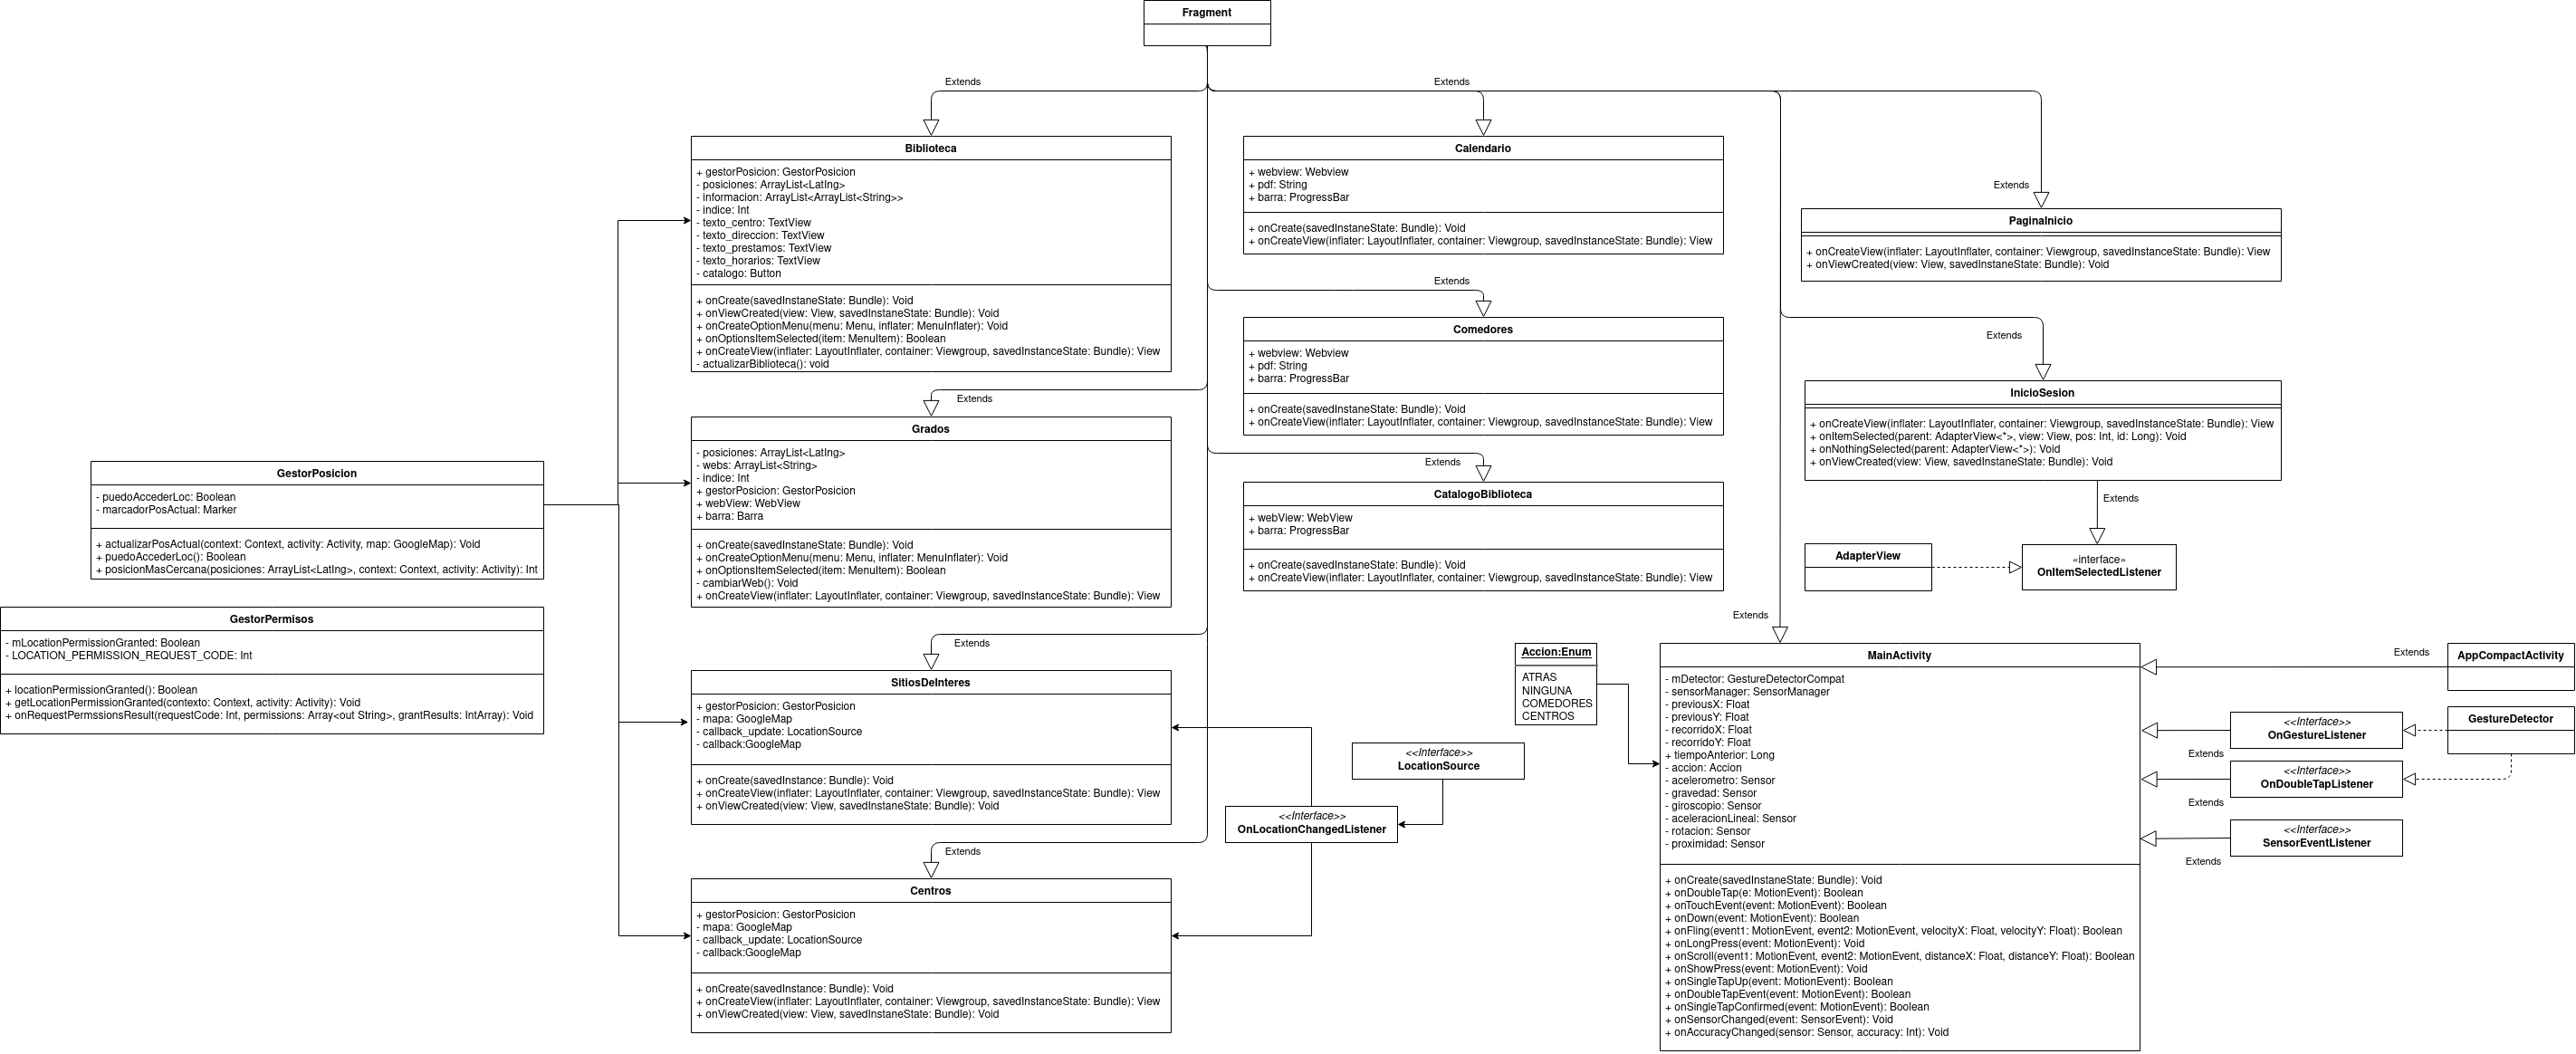
\includegraphics[width=\textwidth]{GuiaEstudiantes.png}
	\caption{Diagrama de Clases del proyecto}
\end{figure}

\newpage
\section{Navigation Graph}

\begin{figure}[H]
	\centering
	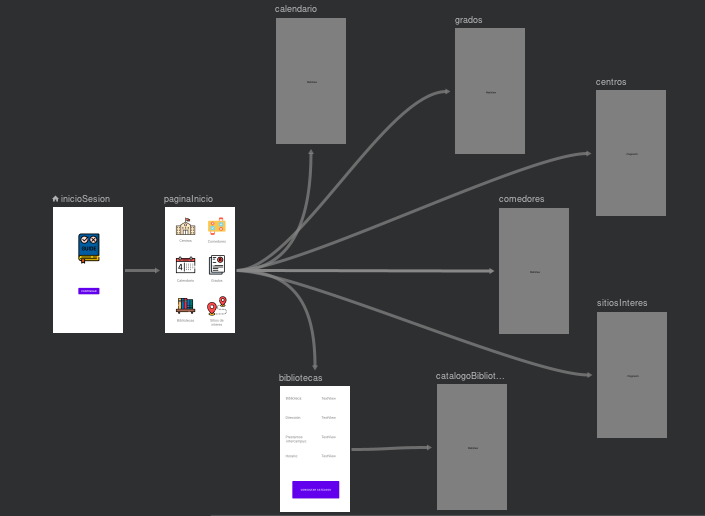
\includegraphics[width=\textwidth]{NavigationGraph.png}
	\caption{Grafo de navegación del proyecto}
\end{figure}

\newpage

\section{Android Manifest}

En este fichero encontraremos información esencial del proyecto, como el nombre del paquete, los permisos que necesita el proyecto, la información sobre nombre, descripción, icono, etc de nuestra aplicación, entre otra información de interes.

En concreto para nuestro caso el paquete será \texttt{com.npi\_grupo4.guiaestudiantes}.

Y debido a las funcionalidades que hemos implementado, se necesitarán los siguientes permisos:

\begin{itemize}

	\item \texttt{android.permission.ACCESS\_FINE\_LOCATION}
	\item \texttt{android.permission.ACCESS\_COARSE\_LOCATION\_LOCATION}
	\item \texttt{android.permission.ACCESS\_COARSE\_LOCATION}
	\item \texttt{android.permission.INTERNET}
	\item \texttt{android.permission.ACCESS\_NETWORK\_STATE}

\end{itemize}

Los tres primeros elementos para tener acceso a la localización y los dos últimos para acceder a internet y a la red del dispositivo.

Otra información de interes que tenemos es la clave de la API de Google Maps, necesaria para que funcionen los fragments de Google Maps, así como que actividad será la actividad principal, donde comenzará la aplicación.



\newpage
\section{Gradle}

El fichero Gradle\cite{gradle} es el fichero de construcción del paquete. Aquí se definirá la forma en la que se construirá el proyecto, desde los plugins con los que trabajamos para desarrollar el proyecto, a que versión de android está dirigido, cuál es la versión de android mínima, con que versión del SDK de android compilaremos y las dependencias necesarias para compilarlo.


En nuestro caso, además del plugin principal de desarrollo en android \texttt{com.android.application} utilizaremos dos plugins para hacer el desarrollo en kotlin más sencillo, \texttt{kotlin-android}\cite{kotlinAndroid} y \\ \texttt{kotlin-android-extensions}.

Con respecto a que versión de android está dirigido el proyecto, debido a que todos los integrantes del grupo disponemos de un teléfono con android 10, el proyecto tiene como objetivo la versión 30 del SDK de android, la correspondiente a android 10, también compilaremos con el SDK 30 de android. Aún así hemos decidido que la versión mínima para ejecutar el proyecto sea el SDK 29, es decir, android 9.0, para realizar pruebas en otros dispositivos.



Como dependencias, tendremos las siguientes:

\begin{itemize}
	\item \texttt{org.jetbrains.kotlin}: Para utilizar como lenguaje de programación Kotlin
	\item \texttt{androidx.core}: Dependencia básica de android.
	\item \texttt{androidx.appcompat}: Dependencia básica de android.
	\item \texttt{com.google.android.material}: Interfaz de Google para android.
	\item \texttt{androidx.constraintlayout}: Dependencia básica de android para gestionar los layout.
	\item \texttt{androidx.navigation}: Dependecia para gestionar la navegación haciendo uso de grafos de navegación.
	\item \texttt{androidx.legacy}: Dependencia básica de android.
	\item \texttt{com.google.android.gms}: API de Google para gestionar la geoposición.
	\item \texttt{com.google.maps.android}: API de Google Maps.
\end{itemize}


En nuestro caso, la mayoría de las funcionalidades se pueden utilizar con la base de android, sin embargo algunas cosas concretas como la geoposición, o gestionar un fragment de Google Map.



\newpage
\section{Fragment Grados}

El objetivo de este fragment es facilitar al usuario que pueda ver las guías docentes de todas las facultades de la UGR.

Para ello vamos a hacer uso principalmente de una \textbf{WebView} que va a cargar las guías docentes apoyándonos en un menú desplegable.

También vamos a hacer uso de una \textbf{ProgressBar} que nos indicará como va el proceso de carga de la url. Vemos necesario usarla porque si no parece que la pantalla no está cargando y el fragment no funciona bien.

A continuación vamos a ver las variables, métodos y funciones que forman este fragment, y que hace cada uno.

\subsection{Variables}

\begin{itemize}

\item{lateinit var webView: WebView}
\item{lateinit var barra: ProgressBar}
\item{private var posiciones = ArrayList$<$LatLng$>$()}
\item{private var webs = ArrayList$<$String$>$()}
\item{private var indice = 0}
\item{var gestorPosicion = GestorPosicion()}

\end{itemize}

Las dos primeras variables son la propia \textbf{WebView} y la \textbf{ProgressBar} de las que he hablado antes. Ambas serán inicializadas en el método \textbf{OnCreateView} usando los id del layout.
La tercera variable corresponde a un ArrayList que guardará las posiciones geográficas de las diferentes facultades de la UGR. La cuarta variable es otro ArrayList que guardará las url de las guías docentes de dichas facultades. La quinta variable es un entero que usaremos para indexar en el ArrayList de url. La última variable es una instancia de la clase \textbf{GestorPosicion()}, la cual usaremos más adelante para calcular la posición geográfica del usuario.

\newpage

\subsection{Métodos}

Los métodos y funciones que voy a explicar a continuación son:

\begin{itemize}
\item{onCreate}
\item{onCreateOptionsMenu}
\item{onOptionsItemSelected}
\item{cambiarWeb}
\item{onCreateView}
\end{itemize}

\subsubsection{Método onCreate}

Esté método empezará indicando que el fragment va a disponer de un menú desplegable usando la orden:

\begin{lstlisting}[language=Kotlin]
setHasOptionsMenu(true)
\end{lstlisting}

Después rellenaremos los ArrayList \textbf{posiciones} y \textbf{webs} con las posiciones geográficas y las url de las guias docentes de las facultades, respectivamente.

\subsubsection{Método onCreateOptionsMenu}

Este método recibe un \textbf{menu} como parámetro y nos encargaremos de añadir a dicho menú las secciones que nos interesen. En este caso, lo rellenaremos con el nombre de las facultades de la UGR. Lo rellenamos de la siguiente forma:

\begin{lstlisting}[language=Kotlin]
menu.add("Facultad de Bellas Artes")
menu.add("E.T.S. de Arquitectura")
menu.add("Facultad de Ciencias de la Educacion")
menu.add("Facultad de Farmacia")
menu.add("Facultad de Medicina")
\end{lstlisting}

\newpage

\subsubsection{Método onOptionsItemSelected}

Este método sirve para indicar que queremos que pase cada vez que el usuario seleccione uno de los elementos del menú desplegable. En nuestro caso vamos a dar un valor u otro a la variable \textbf{indice} dependiendo de la facultad que se seleccione. El indice tendrá el valor necesario para que al indexar en el ArrayList de webs, obtengamos la url de las guias docentes de la facultad que hemos seleccionado.

Después, siempre llamaremos a la función \textbf{cambiarWeb()} que explicaré a continuación.

\subsubsection{Función cambiarWeb}

Cada vez que se llame a esta función, se cargará en la WebView la url correspondiente al valor que tenga \textbf{indice} en ese momento.
Además, se le darán una serie de permisos a la WebView para poder usar JavaScript y acercar/alejar la WebView.

\subsubsection{Método onCreateView}

Este método comienza inicializando las variables \textbf{webview} y \textbf{barra} explicadas anteriormente mediante \textbf{findViewById} y pasándole la Id del layout.

Una vez hecho esto, vamos a configurar la \textbf{WebView} de tal forma que pueda usar JavaScript

\begin{lstlisting}[language=Kotlin]
webview.settings.javaScriptEnabled = true
\end{lstlisting}

y que el usuario pueda usar gestos para acercar y alejar la WebView a su antojo

\begin{lstlisting}[language=Kotlin]
webview.settings.setSupportZoom(true)
webview.settings.builtInZoomControls = true
\end{lstlisting}

También haremos invisible la webview nada más iniciar el fragment para que lo que se vea sea la \textbf{ProgressBar} cargando.

Ahora lo que nos quedaría sería modificar dos objetos internos de nuestra \textbf{WebView}. El primero sería su objeto \textbf{WebChromeClient()}. Este objeto tiene un método llamado \textbf{onProgressChanged} que nos permite ver cómo va el progreso de carga de la WebView, es por esto que lo usaremos para ocultar la webview si el progreso es menor a 100, al mismo tiempo que vamos mostrando como avanza la progressBar. Cuando el progreso llegue a 100, mostraremos la WebView y ocultaremos la ProgressBar.

El otro objeto es el \textbf{WebViewClient()}, el cual tiene un método llamado \textbf{shouldOverrideUrlLoading} y que tiene como parámetro una \textbf{request} que le pasaremos a \textbf{webView.loadUrl(request)}. De esta forma, cada vez que hagamos \textit{"tap"} sobre algún enlace, se recargará la WebView mostrando el enlace. En el caso de intentar cargar un PDF, se hará de manera diferente, ya que nos apoyaremos en la herramienta de visualización de PDF online de Google Drive.

Para terminar, este método calcula cuál es la facultad más cercana al usuario usando la instancia de la clase \textbf{GestorPosicion()}. Así puede cambiar el valor de \textbf{indice} para que las primeras guias docentes que veamos al iniciar el fragment sean las de la facultad más cercana.

\begin{lstlisting}[language=Kotlin]

val pos = gestorPosicion.posicionMasCercana(posiciones,
 requireContext(), requireActivity())

if ( InicioSesion.indice_facultad != -1){
	indice = InicioSesion.indice_facultad
} else if ( pos != null) {
	indice = pos
} else {
	indice = 0
}
cambiarWeb()

\end{lstlisting}

Finalmente nos quedaría mostrar la URL de la guía docente mediante el método \textbf{loadUrl} de nuestra WebView.

\newpage

\begin{figure}[H]
\begin{subfigure}{0.5\textwidth}
  \centering
  % include first image
  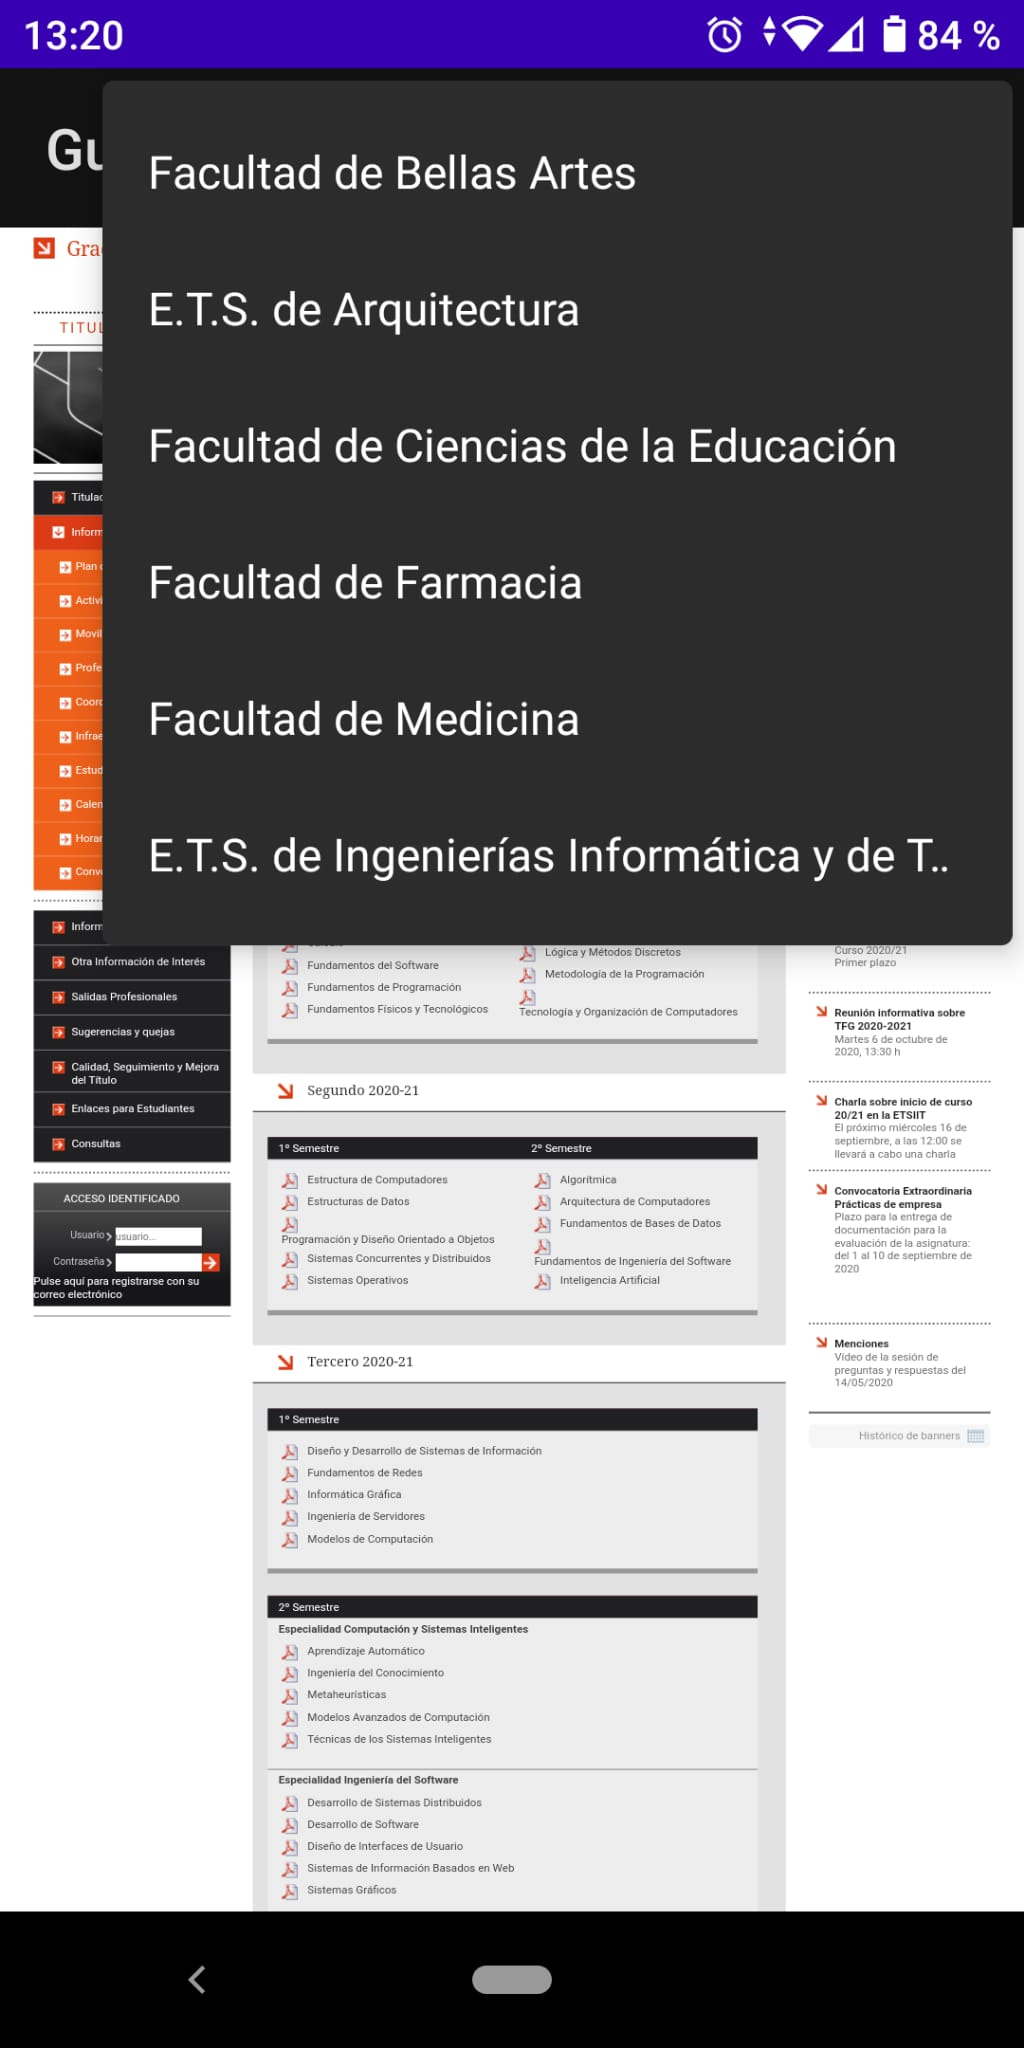
\includegraphics[width=1\linewidth]{menu.jpeg}
  \caption{Menú desplegable}
  \label{fig:sub-first}
\end{subfigure}
\begin{subfigure}{0.5\textwidth}
  \centering
  % include second image
  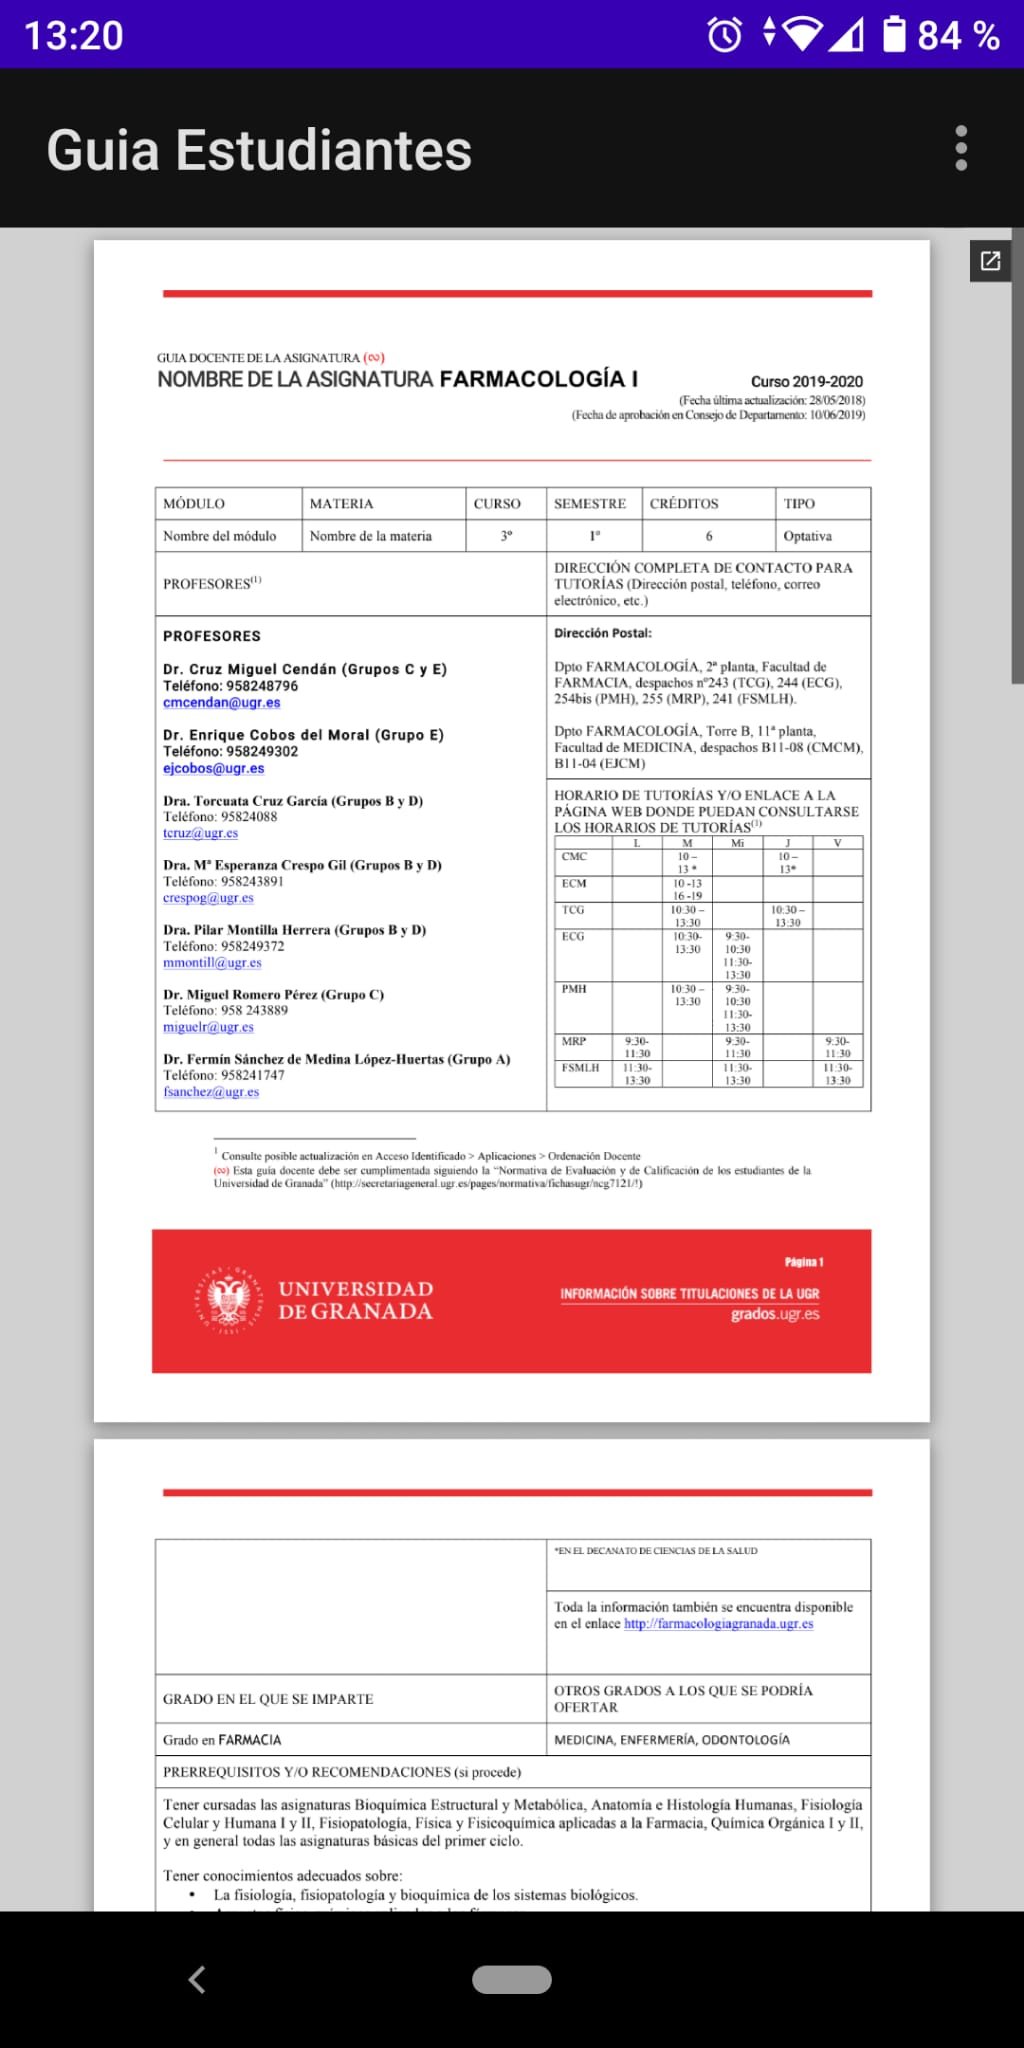
\includegraphics[width=1\linewidth]{guiadocente.jpeg}
  \caption{Guía docente}
  \label{fig:sub-second}
\end{subfigure}
\end{figure}


\newpage
\section{Fragment Comedores}


El objetivo de este fragment es facilitar al usuario que pueda ver el menú semanal que ofrece la UGR en todos sus comedores.

Para ello vamos a hacer uso principalmente de una \textbf{WebView} que va a cargar el pdf \\ \textbf{http://scu.ugr.es/?theme=pdf} apoyándonos en Google Drive.

También vamos a hacer uso de una \textbf{ProgressBar} que nos indicará como va el proceso de carga de la url. Vemos necesario usarla porque si no parece que la pantalla no está cargando y el fragment no funciona bien.

A continuación vamos a ver las variables y los métodos que forman este fragment, y que hace cada uno.

\subsection{Variables}

\begin{itemize}

\item{lateinit var webview: WebView}
\item{lateinit var barra: ProgressBar}
\item{lateinit var pdf: String}

\end{itemize}

Las dos primeras variables son la propia \textbf{WebView} y la \textbf{ProgressBar} de las que he hablado antes. Ambas serán inicializadas en el método \textbf{OnCreateView} usando los id del layout.
La tercera variable corresponde al string que guardará la url de los comedores universitarios y que pasaremos como parámetro al método \textbf{loadUrl} de la WebView.

\newpage

\subsection{Métodos}

Los métodos que voy a explicar a continuación son:

\begin{itemize}
\item{onCreateView}
\end{itemize}

\subsubsection{Método OnCreateView}

Este método comienza inicializando las variables \textbf{webview} y \textbf{barra} explicadas anteriormente mediante \textbf{findViewById} y pasándole la Id del layout.

También le asignamos a \textbf{pdf} la url de los comedores universitarios.

Una vez hecho esto, vamos a configurar la \textbf{WebView} de tal forma que pueda usar JavaScript

\begin{lstlisting}[language=Kotlin]
webview.settings.javaScriptEnabled = true
\end{lstlisting}

y que el usuario pueda usar gestos para acercar y alejar la WebView a su antojo

\begin{lstlisting}[language=Kotlin]
webview.settings.setSupportZoom(true)
webview.settings.builtInZoomControls = true
\end{lstlisting}

También haremos invisible la webview nada más iniciar el fragment para que lo que se vea sea la \textbf{ProgressBar} cargando.

Ahora lo que nos quedaría sería modificar dos objetos internos de nuestra \textbf{WebView}. El primero sería su objeto \textbf{WebChromeClient()}. Este objeto tiene un método llamado \textbf{onProgressChanged} que nos permite ver cómo va el progreso de carga de la WebView, es por esto que lo usaremos para ocultar la webview si el progreso es menor a 100, al mismo tiempo que vamos mostrando como avanza la progressBar. Cuando el progreso llegue a 100, mostraremos la WebView y ocultaremos la ProgressBar.

El otro objeto es el \textbf{WebViewClient()}, el cual tiene un método llamado \textbf{shouldOverrideUrlLoading} y que tiene como parámetro una \textbf{request} que le pasaremos a \textbf{webView.loadUrl(request)}. De esta forma, cada vez que hagamos \textit{"tap"} sobre algún enlace, se recargará la WebView mostrando el enlace.

Finalmente nos quedaría mostrar la URL de los comedores universitarios mediante el método \textbf{loadUrl} de nuestra WebView.

\begin{figure}[H]

  \begin{subfigure}{0.5\textwidth}
    \centering
    % include first image
    \includegraphics[width=1\linewidth]{progressBar.jpeg}
    \caption{Barra de progreso}
    \label{fig:sub-first}
  \end{subfigure}
  \begin{subfigure}{0.5\textwidth}
    \centering
    % include second image
    
\includegraphics[width=1\linewidth]{comedores.jpeg}
    \caption{PDF comedores cargado}
    \label{fig:sub-second}
  \end{subfigure}
\end{figure}


\newpage
\section{Fragment InicioSesion}
Aunque el nombre del insinúe que se se emplea para acceder a una cuenta de usuario, en realidad se trata de un fragmento que permite seleccionar entre una serie de facultades. El nombre se debe a que en el primer prototipo se implementó un inicio de sesión que fue finalmente sustituido, para evitar conflictos y complicaciones se decidió conservar el nombre pero no la funcionalidad original.

Mediante una lista de selección se nos pertmite situar nuestra ubicación predeterminada en una facultad específica. Además, la infomación adicional proporcionada por otros fragmentos, como los horarios de la biblioteca, muestran los de la facultad deseada. También existe la posibilidad de no elegir ninguna y mostrar información de la facultad más cercana.

\subsection{Variables}

\begin{itemize}
	\item indice$\_$facultad
	\item facultad$\_$spinner
	\item boton$\_$continuar
\end{itemize}

\textit{facultad$\_$spinner} es un spinner (lista de selección), mediante un ArrayAdapter le suministramos el string array (facultades) que hemos definido previamente con el nombre de las facultades, junto con la opción ninguna facultad seleccionada, que aparece al principio. Dicho string array está definido en el archivo string.xml.

La variable \textit{indice$\_$facultad} es una variable estática que empleamos para indicar al resto de fragmentos la facultad seleccionada. Cuando seleccionamos una facultad guardamos sus posición en la lista restando 1. Esto es debido a que las ubicaciones de las distintas facultades se almacenan en otra lista. Dicha lista no tiene la opcion ninguna facultad seleccionada. De forma que es necesario restar un 1 para que las posiciones se alineen.

La variable \textit{boton$\_$continuar} es un botón que al interactuar con él nos lleva al fragmento de página de inicio

\newpage
\section{Fragment Centros y Sitios de Interés}
El objetivo de este fragment es mostrar un mapa al usuario de manera que este pueda interactuar con los elementos, así como poder conocer su ubicación a tiempo real y obtener información de los centros e instalaciones de la UGR así como de sitios que puedan ser de interés general.

El motivo de que ambos fragments se traten de manera conjunta es que en cuanto a implementación se refiere ambos están implementados en el proyecto de la misma manera.

Estos fragments funcionan en base al fragment de \textbf{Google Maps}. Utilizamos una clave API solicitada a google para poder acceder a las funcionalidades básicas de los mapas.

Hacemos uso de la ubicación del usuario --- después de previamente solicitar los permisos necesarios --- para mostrar la ubicación de este a tiempo real en un mapa. También utilizamos el \textbf{sensor} de brújula para permitir orientar el mapa según la orientación física del usuario.

El mapa que se muestra en el fragment de centros es un mapa personalizado de google que la UGR pone a disposición de los usuarios con toda la información sobre sus centro y diversas instalaciones.

El mapa utilizado en el fragment sitios de interés se trata de un mapa de google que contiene marcadores en sitios turísticos y de interés general para cualquier persona que visite o desee conocer la ciudad.

A continuación pasaremos a detallar la implementación de ambos fragments:

\subsection{Variables}

\begin{itemize}
	\item gestorPosicion
	\item callback
\end{itemize}

La primera variable \textbf{gestorPosicion} simplemente se encarga de crear una instancia de la clase gestor de posición que resumidamente es la que se encarga de gestionar todos los procesos y rutinas que tienen que ver con la ubicación del usuario.

La variable \textbf{callback} contiene sin embargo una función. Dicha función se ejecutara una vez el mapa haya sido cargado y este listo para ser usado. Esta función se encarga de crear un mapa y centrar la ubicación en la posición del usuario en caso de tener los permisos de ubicación o en una localización por defecto en caso de no tener dichos permisos. Finalmente carga el archivo que contiene los datos del mapa.

\newpage

\subsection{Métodos}
Los métodos implementados por estos fragments son:

\begin{itemize}
	\item onCreate
	\item onOptionsItemSelected
	\item onCreateOptionsMenu
	\item onLocationChanged
	\item onCreateView
	\item onViewCreated
\end{itemize}

\subsubsection{onCreate}
El método onCreate simplemente llama al método onCreate superior de la clase fragment y utiliza
\begin{lstlisting}[language=Kotlin]
setHasOptionsMenu(true)
\end{lstlisting}
para activar la opción de que el fragment tenga un menú de opciones para poder activar o desactivar el sensor de brújula.

\subsubsection{onOptionsItemSelected}
Este método se encarga de activar la brújula una vez se marca el item y de desactivarla si se encuentra activad. Resumidamente conmuta el estado del sensor de brújula.

\subsubsection{onCreateOptionsMenu}
Este método se encarga de crear el menú que permite activar y desactivar la brújula.

\subsubsection{onLocationChanged}
Este método se encarga de llamar a la función del gestor de posición:

\begin{lstlisting}[language=Kotlin]
gestorPosicion.actualizarPosActual(requireContext(), requireActivity(), it)
\end{lstlisting}

cuando detecta un cambio en la ubicación del usuario, lo que permite mantener la misma actualizada a tiempo real.

\subsubsection{onCreateView}
El método onCreateView simplemente se encarga de cargar el fragment de \textbf{Google maps}.

\subsubsection{onViewCreated}
Este método es el que se encarga de solicitar los permisos haciendo uso de la función:

\begin{lstlisting}[language=Kotlin]
GestorPermisos.getLocationPermission(requireContext(), requireActivity())
\end{lstlisting}

Y además se encarga de llamar a la función que almacena la variable \textbf{callback}:

\begin{lstlisting}[language=Kotlin]
mapFragment?.getMapAsync(callback)
\end{lstlisting}

\begin{figure}[H]
\begin{subfigure}{0.5\textwidth}
  \centering
  % include first image
  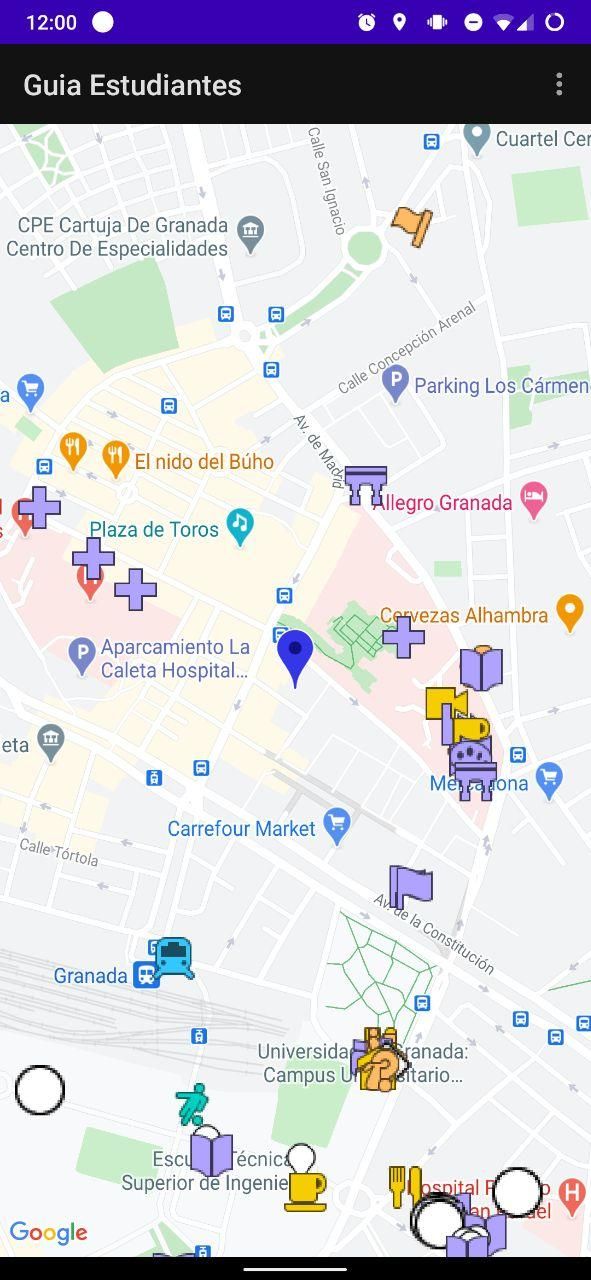
\includegraphics[width=1\linewidth]{centros}
  \caption{Centros}
  \label{fig:sub-first}
\end{subfigure}
\begin{subfigure}{0.5\textwidth}
  \centering
  % include second image
  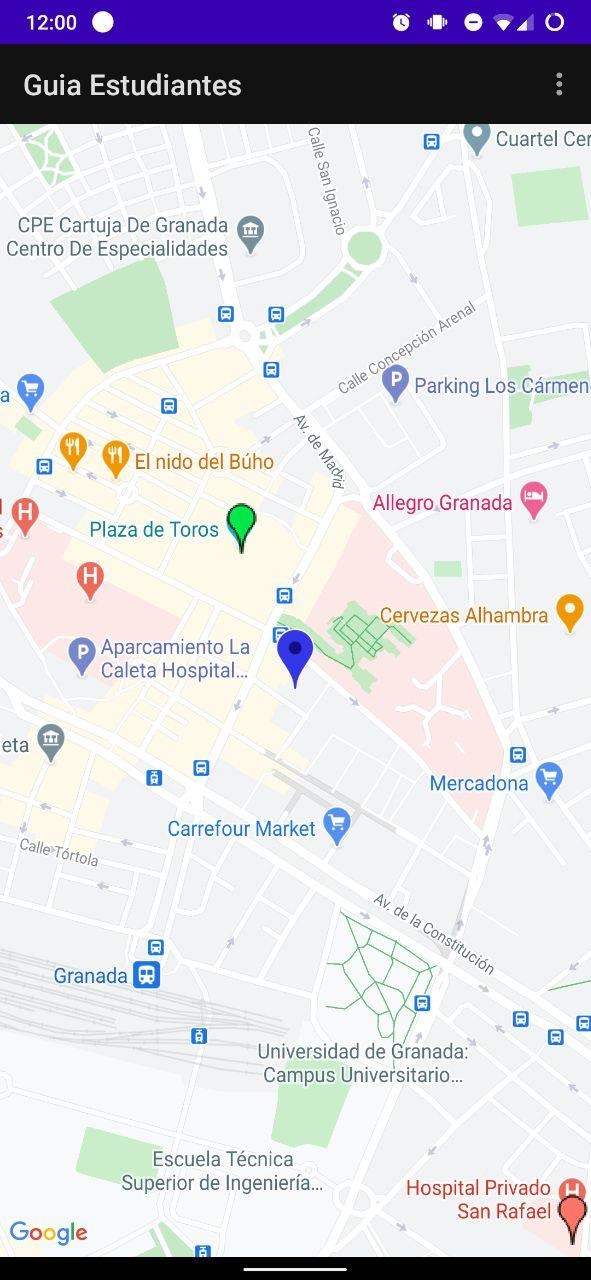
\includegraphics[width=1\linewidth]{sitiosinteres.jpg}
  \caption{Sitios de interés}
  \label{fig:sub-second}
\end{subfigure}
\end{figure}


\newpage
\section{Gestor Posición}

Debido a que varias secciones de nuestro código necesitaban tanto permiso, como funcionalidades relativas a la posición del dispositivo, decidimos crear esta clase con la que poder gestionar este apartado sin tener que repetir código en las distintas clases del proyecto.


Esta clase cuenta con cuatro métodos que son los que hemos utilizado en todo el proyecto.

\begin{itemize}
	\item \texttt{actualizarPosActual(contexto, actividad, mapa)}: Dado un contexto, una actividad y un mapa, actualizar la posición en el mapa dado a la posición actual del dispositivo.
	\item \texttt{rotarMapa(mapa, rotación)}: Dado un mapa, rotar el mapa \texttt{rotación} grados, de forma que el mapa apunte a una orientación dada.
	\item \texttt{getPuedoAccederLoc()}: Devuelve verdadero si puede acceder a la localización del dispositivo, falso en otro caso.
	\item \texttt{posicionMasCercana(posiciones, contexto, actividad)}: Dada una lista de posiciones, devuelve el indice de la más cercana con respecto a la posición del dispositivo.
\end{itemize}


\subsubsection{Método actualizarPosActual}

Este método simplmente utiliza la clase \texttt{LocationServices}\cite{locationServices} para obtener la posición del dispositivo, y si puede acceder, centra el mapa dado a dicha posición, además de añadir un marcador de la posición actual.


\subsubsection{Método rotarMapa}

Haciendo uso de la clase \texttt{CameraPosition}\cite{cameraPosition} de la API de Google Maps, clona los valores de la posición de la camara actual, pero cambiando el atributo \texttt{bearing}, el cual corresponde a la rotación.

Aplica los cambios utilizando el método \texttt{animateCamara}, de forma que si el cambio es brusco aparece como una animación.

\subsubsection{Método getPuedoAccederLoc}

Simplemente devuelve si puede acceder a la ubicación del dispositivo. Verdadero si puedo, falso si no, ya sea por falta de permisos, o porque el dispositivo tiene la localización desactivada.

\subsubsection{Método posicionMasCercana}

Este método obtiene la posición actual, e itera sobre el vector de posiciones dado para encontrar la posición dada más cercana utilizando el método \texttt{distanceBetween} de la clase \texttt{Location}\cite{locationAndroid} de Android.




\newpage
\section{Gestor Permisos}
Utilizamos un objeto en kotlin llamado GestorPermisos con el fin de poder centralizar todos aquellos métodos que necesiten solicitar permisos al usuarios. Los objetos en kotlin son el equivalente a las clases singleton en Java, es decir, objetos que solo pueden instanciarse una sola vez.

\subsection{Variables}
Contamos con dos unicas variables:

\begin{itemize}
	\item mLocationPermissionGranted
	\item LOCATION\_PERMISSION\_REQUEST\_CODE
\end{itemize}

La variable \textbf{mLocationPermissionGranted} simplemente funciona como un flag que indica si los permisos han sido otorgados por el usuario o no. La variable \textbf{LOCATION\_PERMISSION\_REQUEST\_CODE} simplemente es el codigo que le damos a la solucitud de los permisos de ubicación.

\subsection{Métodos}

Este gestor de permisos posee los siguientes métodos:

\begin{itemize}
	\item locationPermissionGranted
	\item getLocationPermission
	\item onRequestPermissionResult
\end{itemize}


\subsubsection{locationPermissionGranted}
Este método simplemente funciona como consultor del valor de la variable \textbf{mLocationPermissionGranted}.

\subsubsection{llocationPermission}
Este es el método que se encarga de solicitar los permisos. Simplemente comprueba uno a uno que los permisos necesarios hayan sido obtenidos correctamente y actualiza el valor de \textbf{mLocationPermissionGranted}.

\subsubsection{onRequestPermissionResult}
Este método se encarga de comprobar que los permisos han sido otorgados y actualizar \textbf{mLocationPermissionGranted} en caso de que no sea asi.



\newpage
\section{Referencias, material y documentación usada}


\begin{thebibliography}{9}

\bibitem{navGraph}

	Navigation Graph - Documentación de Android

	\url{https://developer.android.com/reference/androidx/navigation/NavGraph}

\bibitem{androidManifest}

	Manifiesto de una app - Documentación de Android

	\url{https://developer.android.com/guide/topics/manifest/manifest-intro}

\bibitem{permisosManifest}

	Permisos de un proyecto Android - Documentación de Android

	\url{https://developer.android.com/guide/topics/manifest/uses-permission-element?hl=es-419}

\bibitem{gradle}

	Ficheros Gradle y sugerencias - Documentación de Android

	\url{https://developer.android.com/studio/build/gradle-tips?hl=es}

\bibitem{kotlinAndroid}

	Kotlin para desarrollo Android - Documentación de Kotlin

	\url{https://kotlinlang.org/docs/reference/android-overview.html}

\bibitem{webView}

	Uso de WebView en Android - Documentación de Android

	\url{https://developer.android.com/guide/webapps/webview}

\bibitem{menusAndroid}

	Menús en Android - Documentación de Android

	\url{https://developer.android.com/guide/topics/ui/menus?hl=es-419}

\bibitem{activityAndroid}

	Clase Activity en Android - Documentación de Android

	\url{https://developer.android.com/reference/android/app/Activity}

\bibitem{sensorAndroid}

	SensorManager en Android - Documentación de Android

	\url{https://developer.android.com/reference/android/hardware/SensorManager}

\bibitem{tiposSensoresAndroid}

	Tipos de sensores en Android - Documentación de Android

	\url{https://developer.android.com/guide/topics/sensors/sensors_overview}

\bibitem{cameraPosition}

	CameraPosition - Documentación de la API de Google Maps

	\url{https://developers.google.com/android/reference/com/google/android/gms/maps/model/CameraPosition}

\bibitem{locationServices}

	Servicios de localización - Documentación de la API de Google Maps

	\url{https://developers.google.com/android/reference/com/google/android/gms/location/LocationServices}


\bibitem{locationAndroid}

	Clase Location - Documentación de Android

	\url{https://developer.android.com/reference/android/location/Location}

\end{thebibliography}



%%%%%%%%%%%%%%%%%%%%%%%%%%%%%%%%%%%%%%%%%%%%%%%%%%%%%%%%%%%%%%%%%%%%%%%%%%%%%%%%%%%%%%%%%


\end{document}
